\section{Challenging localization scenario}
\label{sec:chall_loc}

\subsection{Night to day localization}
\label{subsec:night2day}

Night to day localization is an extremely challenging problem: our best RGB baseline achieves less than 13\% recall@1. This can be explained by the huge difference in visual appearance between night and daytime images, as illustrated in figure~\ref{fig:dataset}. Our system should be able to improve the RGB baseline relying on the learned scene geometry, which remains the same during day and night. Unfortunately, we use training data exclusively composed of daytime images, thus making the decoder unable to reconstruct a depth map from an image taken at night. The last line of figure~\ref{fig:mod_ex} shows the poor quality of decoder output after initial training. In order to improve the decoder's performances, we propose to use weakly annotated data to fine tune the decoder part of our system. We collect 1000 pairs of image and depth map acquired at night and retrain only decoder weights $\theta_G$ using loss of equation~(\ref{eq:l1_loss}). Figure~\ref{fig:mod_ex} presents the qualitative amelioration on the inferred depth map after the fine tuning. Such post-processing trick cannot be used to improve standard RGB image descriptors, because we need to know the location of the night data. For instance, we use a night run from the Robotcar dataset with a low quality GPS signal, that makes impossible the automatic creation of triplets that are essential for training a deep image descriptor. 

We show in figure~\ref{fig:ft_night}-c that we are able to nearly multiply by two the localization performances by only fine tuning a small part of our system. Our best network achieves 23\% recall@1 against 13\% recall@1 for the best RGB baseline.

\begin{figure}
%	\includegraphics[trim={0 15 0 0},clip,width=\linewidth]{vect/mod_ex}	
	\centering
	
	\begin{minipage}{0.15\linewidth}
		\center\scriptsize
		Images
	\end{minipage}\hfill
	\begin{minipage}{0.84\linewidth}
	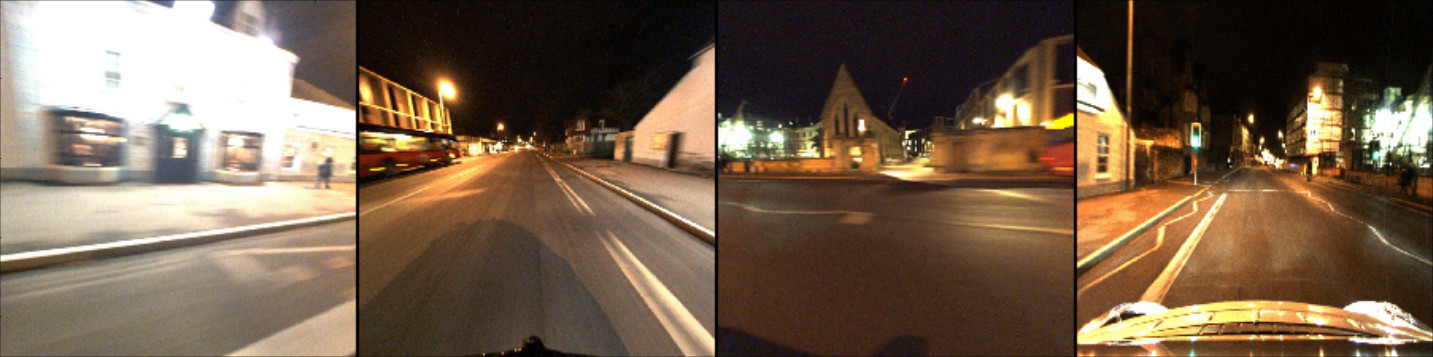
\includegraphics[width=\linewidth]{chall_loc/depth_night_im/input}		
	\end{minipage}
	
	\begin{minipage}{0.15\linewidth}
		\center\scriptsize
		Ground truth depth map
	\end{minipage}\hfill
	\begin{minipage}{0.84\linewidth}
	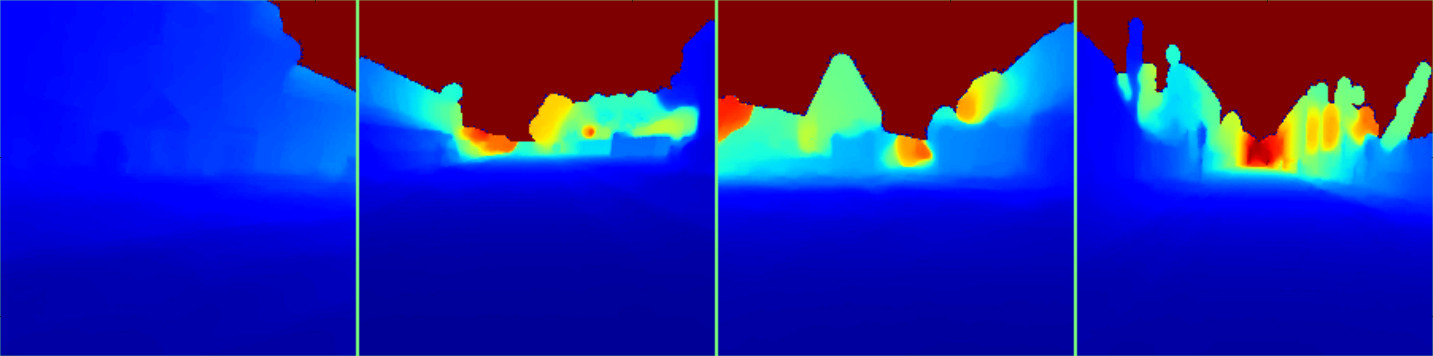
\includegraphics[width=\linewidth]{chall_loc/depth_night_im/gt}	
	\end{minipage}
	
	\begin{minipage}{0.15\linewidth}
		\center\scriptsize		
		Generated depth map after fine tuning
	\end{minipage}\hfill
	\begin{minipage}{0.84\linewidth}
	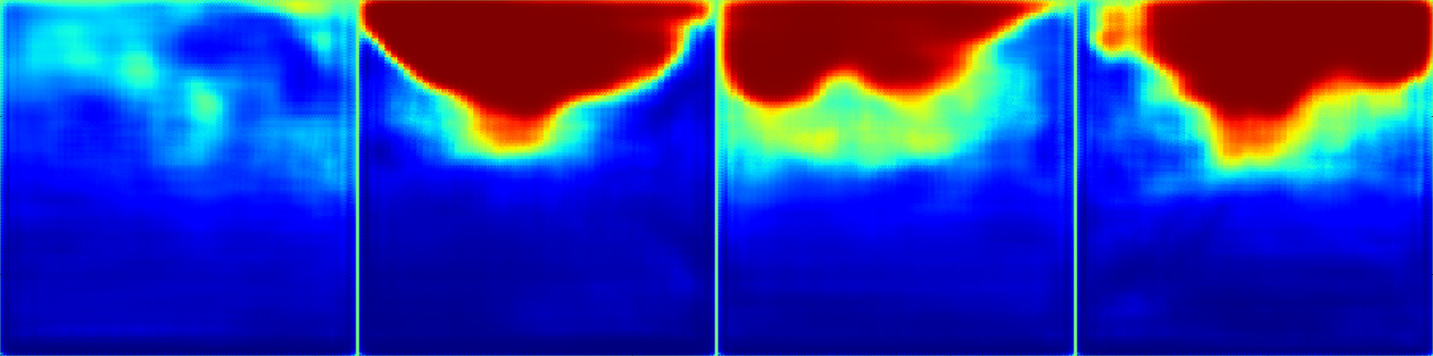
\includegraphics[width=\linewidth]{chall_loc/depth_night_im/ft}	
	\end{minipage}

	\begin{minipage}{0.15\linewidth}
		\center\scriptsize		
		Generated depth map before fine tuning
	\end{minipage}\hfill
	\begin{minipage}{0.84\linewidth}
	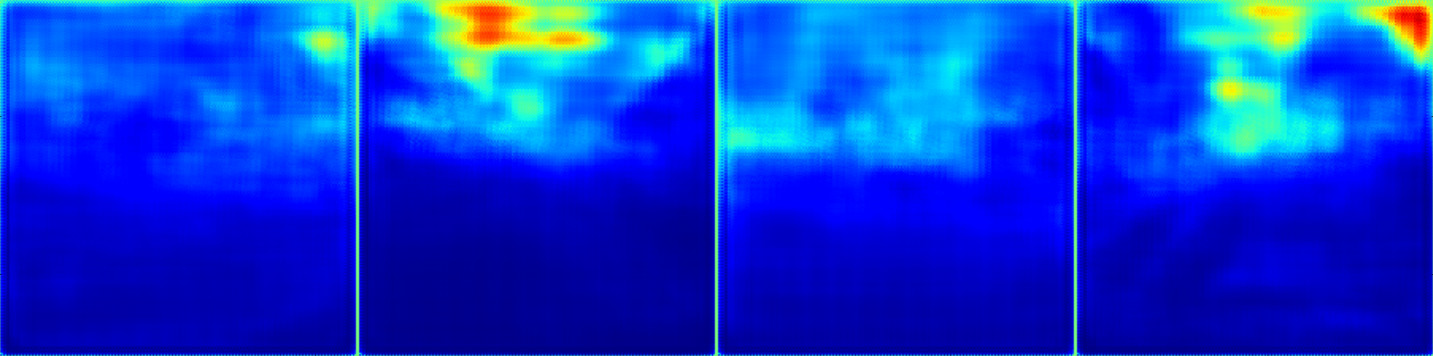
\includegraphics[width=\linewidth]{chall_loc/depth_night_im/noft}	
	\end{minipage}
	
	\caption[Effect of fine tuning with night images on decoder output]{\label{fig:mod_ex} \textbf{Effect of fine tuning with night images on decoder output:}. Decoder trained with daylight images is unable to reconstruct the scene geometry (bottom line). Fine tuning the network with less than 1000 pairs \{image, depth map\} acquired by night highly improves appearance of the generated depth maps. Maps best viewed in color.}
	
\end{figure}

\begin{figure}
	\center
	\begin{minipage}{0.27\linewidth}
		\center \scriptsize
		\includegraphics[width=\linewidth]{plot/night_ft/Results_lt_queries/distance}	
		
		\includegraphics[width=\linewidth]{plot/night_ft/Results_lt_queries/recall}
		
		a) Oxford -- LT
	\end{minipage}
	\begin{minipage}{0.27\linewidth}
		\center \scriptsize
		\includegraphics[width=\linewidth]{plot/night_ft/Results_snow_queries/distance}	
		
		\includegraphics[width=\linewidth]{plot/night_ft/Results_snow_queries/recall}
				
		b) Oxford -- Snow
	\end{minipage}
	\begin{minipage}{0.27\linewidth}
		\center \scriptsize
		\includegraphics[width=\linewidth]{plot/night_ft/Results_night_queries/distance}	
		
		\includegraphics[width=\linewidth]{plot/night_ft/Results_night_queries/recall}
		
		c) Oxford -- Night
	\end{minipage}

	\vspace{5pt}	
	
	\begin{minipage}{0.27\linewidth}
		\center \scriptsize
		\includegraphics[width=\linewidth]{plot/night_ft/Results_cmu_lt/distance}	
		
		\includegraphics[width=\linewidth]{plot/night_ft/Results_cmu_lt/recall}
		
		d) CMU -- LT
	\end{minipage}
	\begin{minipage}{0.27\linewidth}
		\center \scriptsize
		\includegraphics[width=\linewidth]{plot/night_ft/Results_cmu_snow/distance}	
		
		\includegraphics[width=\linewidth]{plot/night_ft/Results_cmu_snow/recall}
		
		e) CMU -- Snow
	\end{minipage}
	\begin{minipage}{0.27\linewidth}
		\center \scriptsize
		\includegraphics[width=\linewidth]{plot/night_ft/Results_cmu_autumn/distance}	
		
		\includegraphics[width=\linewidth]{plot/night_ft/Results_cmu_autumn/recall}
		
		f) CMU -- Autumn
	\end{minipage}
	
	\vspace{0.2cm}
		
	\begin{scriptsize}
	\begin{tabular}{c l c l}
		\textcolor{blue}{\textbf{--}} & Alexnet RGB(D) & \textcolor{cyan}{\textbf{--}} & Alexnet RGB(D) fine tuned \\
		\textcolor{blue}{\textbf{- -}} & Resnet RGB(D) & \textcolor{cyan}{\textbf{- -}} & Resnet RGB(D) fine tuned \\
	\end{tabular}		
	\end{scriptsize}
	
	\caption[Results after fine tuning]{\label{fig:ft_night} \textbf{Results after fine tuning:} we are able to drastically improve localization performance for the Oxford -- Night challenging scenario (c) by only fine tuning the decoder part of our network with weakly annotated data. Curves best viewed in color.}
\end{figure}


\subsection{Influence on over environments}
\label{subsec:night2day_inf}
In this section we measure the influence of the fine tuning process on over localization scenarios. Performances could decrease if our system \textit{``forgets''} how to produce depth map from daylight images. To prevent that, we integrate half of daylight images with the night images in the training data used for fine tuning. 

We show results of the fine-tuned network on figure~\ref{fig:ft_night}. Localization accuracy remains stable after the fine tuning. We even observe slight increase in the localization performances for some scenario (figure~\ref{fig:ft_night}-b): thank to the fine tuning with night images, the decoder had improved the depth map generation of dark images acquired during daytime. The fact that fine tuning our system to deal with hard localization scenario do not negatively impact the performances on over environment makes our new method well suited for real application when we cannot predict what will be the outdoor conditions.

